\subsubsection{Q10.20 data 09202021 10082021 10312021 11092021 grouped by scenario \& PGM}

\begin{comment}
                             EFPR        EO      EFNR     n    pvalue
(frauth, Advantaged)     0.526786  0.473214  0.455357  56.0  0.555439
(frauth, Disadvantaged)  0.404762  0.595238  0.523810  21.0  0.287938
(icu, Advantaged)        0.621622  0.378378  0.567568  37.0  0.056030
(icu, Disadvantaged)     0.481481  0.518519  0.685185  27.0  0.950828
(rent, Advantaged)       0.397059  0.602941  0.426471  34.0  0.297320
(rent, Disadvantaged)    0.486842  0.513158  0.447368  38.0  0.946217
\end{comment}

\begin{table}[h]
    \centering
    \begin{tabular}{|c|c|c|c|c|c|c|}
        \hline
        scenario & PGM & EFPR & EO & EFNR & n & p-value\\
        \hline
        frauth & Advantaged & \textbf{0.527} & 0.473 & 0.455 & 56.0 & 0.555\\
		frauth & Disadvantaged & 0.405 & \textbf{0.595} & \textbf{0.524} & 21.0 & 0.288\\
		icu & Advantaged & \textbf{0.622} & 0.378 & \textbf{0.568} & 37.0 & 0.056\\
		icu & Disadvantaged & 0.481 & \textbf{0.519} & \textbf{0.685} & 27.0 & 0.951\\
		rent & Advantaged & 0.397 & \textbf{0.603} & 0.426 & 34.0 & 0.297\\
		rent & Disadvantaged & 0.487 & \textbf{0.513} & 0.447 & 38.0 & 0.946\\
		
        \hline
    \end{tabular}
    \caption{Grouped by scenario PGM}
    \label{tab:my_label}
\end{table}
\begin{figure}[h]
    \centering
    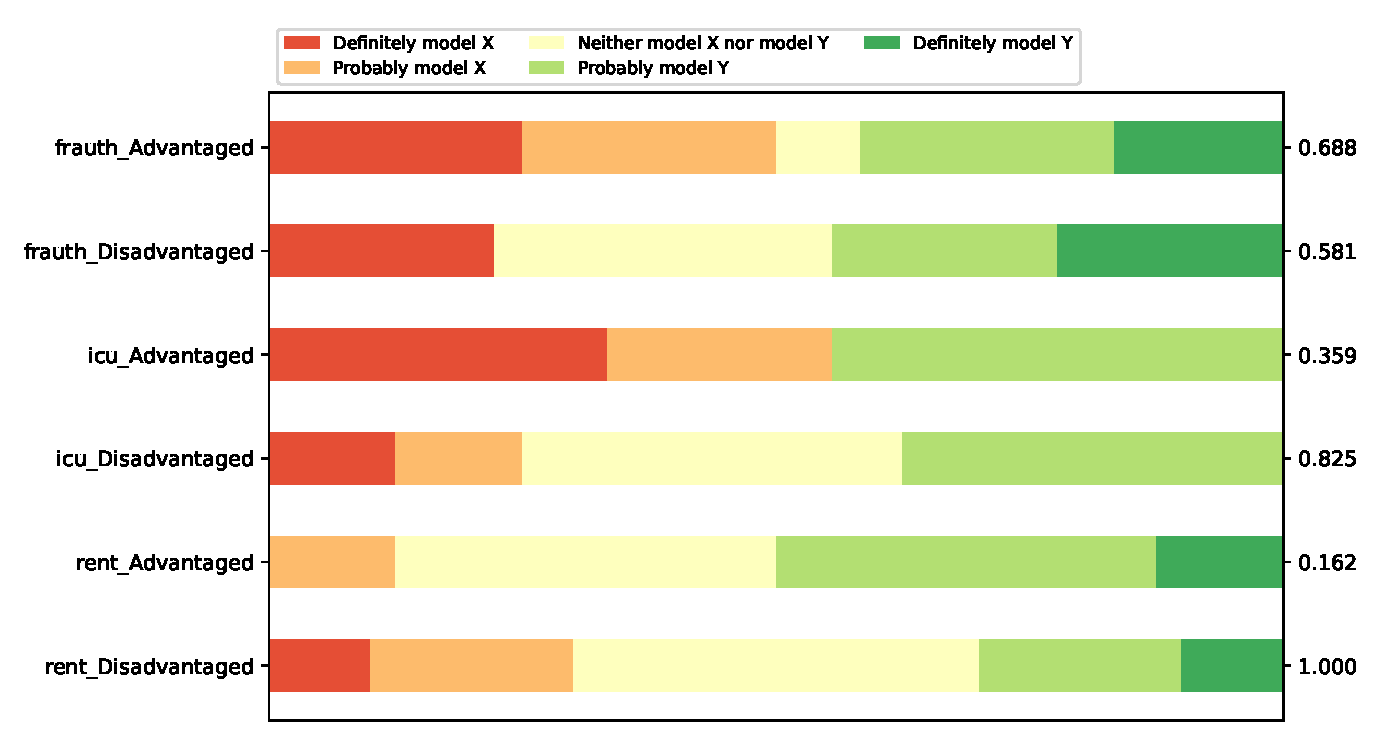
\includegraphics[width=0.8\textwidth]{figures/Q10.20/09202021_10082021_10312021_11092021/Q10.20_scenario_PGM.pdf}
    \caption{Grouped by scenario \& PGM}
    \label{fig:my_label}
\end{figure}
